\def\baselinestretch{1}
\chapter{Poem Analysis}
\ifpdf
    \graphicspath{{Theory/TheoryFigs/PNG/}{Theory/TheoryFigs/PDF/}{Theory/TheoryFigs/}}
\else
    \graphicspath{{Theory/TheoryFigs/EPS/}{Theory/TheoryFigs/}}
\fi

\def\baselinestretch{1.66}

The first phase of implementation involves writing a suite of algorithms to analyse a single poem in terms of the features mentioned in section \ref{sec:features}. The aim is to run a large collection of poems through this analysis to learn the usage patterns of poetic features for any collection of poems. This is in line with the ultimate aim of generating poems without hard-coded rules for different types of poems.

The algorithms will cover the detection of the use of:
\begin{itemize}
\setlength{\itemsep}{0pt}
\item{Rhyme and internal rhyme}
\item{Rhythm, including meter and syllable count}
\item{Alliteration, assonance, consonance, onomatopoeia and other sound devices}
\item{Structure, tense, point of view and repetition}
\end{itemize}

Other algorithms will attempt to understand the context of the poem to extract:
\begin{itemize}
\setlength{\itemsep}{0pt}
\item{Characters}
\item{Objects}
\item{Locations}
\item{Descriptions}
\item{Relationships}
\item{Actions}
\item{Symbolism including metaphors, similes and personification}
\end{itemize}

The output of this phase is a full analysis of a single poem. In lieu of this, we will walk through the implementations of each of these algorithms using the poems in Figures \ref{fig:cat} and \ref{fig:limerick} as case studies.


\begin{figure}
\centering
\begin{minipage}{0.45\textwidth}
\centering
\textit{
There once was a big brown cat\\
That liked to eat a lot of mice.\\
He got all round and fat\\
Because they tasted so nice.
}
\caption{A rhyming quatrain often used in teaching poetry}
\label{fig:cat}
\end{minipage}\hfill
\begin{minipage}{0.45\textwidth}
\centering
\textit{
The limerick packs laughs anatomical\\
Into space that is quite economical.\\
    But the good ones I've seen,\\
    So seldom are clean,\\
And the clean ones so seldom are comical.
}
\caption{A limerick about limericks}
\label{fig:limerick}
\end{minipage}
\end{figure}


\section{Obtaining Phonetic Structure}
\label{sec:phonetic}
Poets choose words based the \textit{sound} when spoken out loud as well as their (literal or symbolic) meaning. As explained in section \ref{sec:words}, we can use Carnegie Mellon University Pronounciation Dictionary (CMUPD) to get around the difficulty of determining phonetic structure. A word in the CMUPD is mapped to a list of different pronunciations for the same word. Each pronunciation is a list of phonemes that make up that particular pronunciation of that word, including indication of emphasis on the syllables.

We want to convert the poems into their pronunciations for use by the detection algorithms. This needs to be done word by word, so we first need to \textit{tokenise} the sentence. Tokenisation involves splitting each sentence into a list of its basic components; words and punctuation. Once we have that, we iterate through the list and run each word through the CMUPD. Some words have multiple pronunciations, so we consider each possible permutation of pronouncing each line of the poem. Each of the pronunciations of the first line of Figure \ref{fig:cat} is shown in Figure \ref{fig:catpronun}.

\begin{figure}
\centering
{[ DH EH1 R ]}\\
{[ W AH1 N S ]}\\
{[ W AA1 Z ], [ W AH1 Z ], [ W AH0 Z ], [ W AO1 Z ]}\\
{[ AH0 ], [ EY1 ]}\\
{[ B IH1 G ]}\\
{[ B R AW1 N ]}\\
{[ K AE1 T ]}
\caption{The different ways of pronouncing the first line of the cat poem}
\label{fig:catpronun}
\end{figure}

Unfortunately, the CMUPD only has about 133,000 words. This means that we are occasionally unable to translate to the phonetic structure, particularly in Shakespearean poems. We get around this by temporarily converting the word into its closest match that exists in the dictionary and returning the phonetic structure in its place.

Python \textit{difflib}\cite{difflib} provides a function to find the closest matches of a word to a list of words, based on the Ratcliff/Obershelp pattern recognition algorithm. The complexity of this algorithm is quadratic in the worst and average case, linear in the best case. 

The behaviour is based on  how many subsequences the words have in common. Since we are only dealing with single words at a time, we have a higher chance of the best case. On average it takes 0.81 seconds to look up a 4-letter word and 1.09 seconds to look up a 10-letter word using machine specifications given in Appendix \ref{sec:specs}, which is fast enough given that this is a pre-processing phase, not a time-sensitive one.

We could use a variety of other techniques to get around this problem other than string matching:
\begin{itemize}
\item{Break many syllable words into likely part-words, e.g. \textit{'thrift'} and \textit{'less'} instead of \textit{'thriftless'}.}
\item{Try all combinations of stress and syllables.}
\item{Train a finite-state transducer model as in Dobrivsek et al. 2010\cite{dobrivsek2010towards}.}
\end{itemize}

The first option only works in a limited number of situations, most of which are handled by the string matching solution. For example, \textit{'thriftless'} would become \textit{'shiftless'}, which has an identical phonetic structure. The second option can result in poor performance and more false negatives or false positives than would be worth the added processing.

The final option is the most viable and would be used if the generation phase depended on perfect readings of the poems, such as in the stochastic n-gram methodology of RKCP (section \ref{sec:RKCP}). We only need an approximation for each individual poem because our results will depend on the analysis of a large number of poems, which will reduce the bias caused by any anomalies.


\section{Rhyme}

We want to detect end-line and internal rhyme, as described in section \ref{sec:rhyme}. We want to be able to build a normalised rhyme scheme representation for easy analysis in the abstraction phase. 

First we collect the pronunciations of the words for which we wish to build a rhyme scheme. For end-line, we collect the last word of each line of the poem. For internal rhyme, we collect the all the words in a particular stanza.

Once we have our list, we can run it through Algorithm BLAH.

1 for each word in the list:\\
2 	for each pronunciation of the word:\\
3		for each phoneme in the pronunciation:\\
4			if this phoneme is stressed:\\
5				get the tail of the pronunciation from this phoneme onwards\\
6				get the rhyme phoneme pattern of this tail\\
7				if we have seen this pattern before: \\
8					assign it the corresponding rhyme token\\
9				else:\\
10					assign this pattern a new rhyme token\\
11				\\
12				append this token to a set of possible tokens for this word\\				
13	append the set of possible tokens for this word to the unzipped rhyme scheme\\
14 build all possible permutations of rhyme scheme from they unzipped rhyme scheme\\
15 normalise the rhyme schemes\\
	
There are a few tricks to this algorithm, namely obtaining the rhyme phoneme pattern on line 6 and the process of building and normalising the rhyme scheme in lines 12 to 15. These processes are explained in the coming sections.

\subsection{Obtaining the Rhyme Phoneme Pattern}

Words rhyme when both of the following conditions are met:
\begin{itemize}
\item{the last phoneme of each word match}
\item{the vowel sounds after and including the first \textit{stressed} syllable match \textbf{in order}}
\end{itemize}

The algorithm finds the first stressed syllable in line 4. At that point we only need to iterate through the rest of the pronunciation, checking the vowel sounds and the last phonemes. Putting them together, in order, gives the unique rhyme phoneme pattern. 

For EXAMPLE strategy and tragedy, kite and height - colourful diagrams!			

\subsection{Building and Normalising the Rhyme Scheme}

Each unique rhyme phoneme pattern is represented by a single capital letter starting with 'A'. This is the standard convention for rhyme schemes used in literary theory. 

The fact that a single word may have several pronunciations creates a complication. To cope with it, we create a tuple for every possible rhyme pattern for a each word. The list of these tuples is what the algorithm refers to as the 'unzipped' rhyme scheme on line 12 and 13. Figure BLAH shows the unzipped rhyme scheme for the limerick in Figure BLAH. Note that the word \textit{'anatomical'} has two pronunciations that affect the rhyme pattern, according to the CMUPD.

FIGURE OF THE UNZIPPED RHYME SCHEME

We then build every possible permutation of this list, which then gives us all of the possible rhyme schemes for the given words. We leave this list as it is and do not make a claim for any rhyme scheme to be more likely than any other at this stage.

EXAMPLE RHYME SCHEMES OF CAT AND LIMERICK

\section{Rhythm}

We attempt to recognise all three types of rhythm described in \ref{sec:rhythm}. 

\subsection{Detecting Syllabic Rhythm}

The number of syllables in a word is equal to the number of vowel phonemes it has. We know that all vowel phonemes have a stress marker appended to them so counting the number of stress markers in the word will give us the number of syllables.

Syllabic rhythm is done on a line-by-line basis, so we tokenise each line and aggregate the syllables across all words in the line.

If we take one permutation of the line in Figure \ref{fig:catpronun}, we can see that each word has one vowel phoneme, i.e. each word in that sentence is monosyllabic. Therefore the number of syllables in the line is 7.

The full syllabic rhythm for the poems in Figure \ref{fig:cat} and \ref{fig:limerick} are 7-8-6-7 and 11-6-5-11-11 respectively. We represent these as a tuple of integers and create a separate list of them for each stanza.

\subsection{Detecting Quantitative and Accentual Rhythm}

While theory counts rhythm in terms of metre and feet, as described in \ref{sec:rhythm}, some poems might have rhythm without following one of these pre-defined popular styles. Instead of searching for them specifically, we will extract the pattern of stressed and unstressed syllables for each line without making a claim on how it matches to theory.

We choose to do this mainly because there could be multiple possibilities for the stress pattern of a line due to variations in emphasis for particular words, e.g. \textit{'\textbf{ob}ject'} and \textit{'ob\textbf{ject}'}. The variability of possible stress patterns is compounded by limitations of the CMUPD:
\begin{itemize}
\item{Some words are restricted to a single stress pattern even though it does not lose or change the meaning of the word if it was emphasised differently. For example, \textit{'\textbf{quan}tity'}, \textit{'quan\textbf{ti}ty'} and \textit{'quanti\textbf{ty}'} are all valid, but the CMUPD only recognises the first because the other two are unusual in normal speech, but not necessarily for poetry.}
\item{Similarly, the CMUPD fixes monosyllabic words to one of stressed or unstressed as in Figure \ref{fig:catpronun}. In poetry, however, they can be either so we need to allow for both possibilities.}
\item{Stresses on some words have changed over time. For example \textit{\textbf{prov}ed} was pronounced \textit{prov\textbf{ed}} in Shakespeare's era.}
\item{Though not necessarily a limitation, we do not recognise light or secondary stress in a word (the '2' stress marker). We therefore assume it could be either '1' or '0'.}
\item{Poetic license often allows words to be pronounced with an entire extra syllable. For example \textit{'de-served'} could be pronounced as \textit{'de-ser-ved'}.}
\end{itemize}

We account for these by manually increasing the possible phonetic stress marker readings. Unfortunately, this will lead to an unrealistically large number of possibilities. For example, the line in Figure \ref{fig:catpronun} will give us all combinations of '1's and '0's. 

We narrow this down by taking away any occurrences of the same stress three or more times in a row in the same line because it will never be read this way.  

Like with rhyme, we do not make a claim for any stress pattern to be more likely than any other at this stage.

FIGURE of possible stress patterns for first line of cat and limerick


\section{Sound Devices}

We aim to detect each of the sound devices described in \ref{sec:sound}; alliteration, assonance and consonance.

The implementation for all three of them is very similar. For each line, we map each phoneme to the number of times it occurs and return those that occur more than once.

The only difference is that assonance only looks at \textit{vowel} phonemes (i.e. with a stress marker) and consonance only looks at \textit{non-vowel} phonemes. Alliteration only looks at either the \textit{first} phoneme of each word in the line, or the \textit{first stressed} phoneme and the one \textit{immediately before} that.

For example, take the phrase \textit{"Slither slather"}:
\begin{itemize}
\item{\textbf{Consonance}: The phonemes \textit{'S'}, \textit{'L'} and \textit{'DH'} occur twice.}
\item{\textbf{Assonance}: The phoneme \textit{'ER0'} occurs twice.}
\item{\textbf{Alliteration}: The phonemes \textit{'S'} and \textit{'L'} occur twice each at the start of the word.}
\end{itemize}

Common phrases like \textit{'take away'} would give an assonance score on the \textit{'EY1'} phoneme, which may not be intended. Therefore, we put a condition that we the occurrence counts for each sound device must be greater than 2. For example, consonance has a total occurrence score of six, assonance of two and alliteration of four. Therefore, the assonance would not be recognised.

Take another example: \textit{"Mammals named Sam are clammy"}
\begin{itemize}
\item{\textbf{Consonance}: \textit{'M'} occurs five times while \textit{'L'} occurs twice.}
\item{\textbf{Assonance}: The phoneme \textit{'AE1'} occurs thrice.}
\item{\textbf{Alliteration}: None.}
\end{itemize}

\section{Form}

We implement some detectors for the form and structure of the poem. This does not include analysis of words and phrases themselves as that will be done in the next phase, as described in section BLAHINTHEINTERPRETATION.

\subsection{Structure and Repetition}

The algorithms for detecting the features of structure described in section \ref{sec:structure} are:

\begin{description}
\item[Number of stanzas] \hfill \\
Count blank lines and add 1
\item[Number of lines per stanza] \hfill \\
Count new line characters of each stanza
\item[Number of distinct sentences] \hfill \\
The number of sentences returned when parsed using the CLiPS\cite{de2012pattern} \textit{parsetree} function. 
More lines than sentences indicates \textbf{enjambment}.
\item[Number and location of repeated lines] \hfill \\
Find the list of non-unique lines. For each of those lines, find its line number locations in the poem.

\end{description}

The poem in Figure \ref{fig:cat} has one stanza, four lines, no repeated lines and two distinct sentences, indicating enjambment.

The poem in Figure \ref{fig:limerick} has one stanza, five lines, no repeated lines and four distinct sentences, indicating enjambment.

\subsection{Point of View}

We can also determine the point of view of the speaker, i.e. whether it is in first or third person. If we find the word \textit{'I'} anywhere in the poem and as long as it is outside speech marks, we say that the entire poem is in first person. Otherwise we default to third person. Figure \ref{fig:cat} is written in third person but Figure \ref{fig:limerick} is in first person.

\subsection{Tense}

The tense of each line can be found by analysing the verb in that sentence. CLiPS pattern library provides a method of doing this using their \textit{'tenses'} function. It also gives us the \textit{aspect}, e.g. perfect, progressive. However, tests found this to be less accurate so we will settle for just the tense.

We record the tense of each line as well as the overall tense of the poem. Each line in the cat poem in Figure \ref{fig:cat} is in past tense giving a past tense overall. The limerick in Figure \ref{fig:limerick} is in present tense overall because all but one line, is in present tense. 


\section{Characters and Context}
Here we describe our approach to determining the context of the poem in terms of its characters and their relationships as described in section \ref{sec:pragpers}. The aim is to build a representation of the characters much like the conceptual networks described in Section \ref{sec:common-sense-bg}. This will then be compared in the abstraction phase to find a correlation between these representations and collections of poetry.

\subsection{Semantic Relations}
The semantic relations between persona in this project are based on those used in ConceptNet, the semantic network of and general knowledge described in Section \ref{sec:conceptnet}. We can use the following relations to build our desired representation.

\begin{description}
\item[MadeOf] \hfill \\ What is it made of? \hfill \\ E.g. tree - MadeOf $\rightarrow$ wood
\item[IsA] \hfill \\ What kind of thing is it? \hfill \\ E.g. banana - IsA $\rightarrow$ fruit
\item[AtLocation] \hfill \\ Where would you find it? \hfill \\ E.g. priest - AtLocation $\rightarrow$ church
\item[CapableOf] \hfill \\ What can it do? \hfill \\ bird - CapableOf $\rightarrow$ sing
\item[Desires] \hfill \\ What does it want? \hfill \\ banker - Desires $\rightarrow$ his loan to be repay
\item[HasA] \hfill \\ What does it have in its possession? \hfill \\ old person - HasA $\rightarrow$ white hair
\item[HasProperty] \hfill \\ What properties does it have? \hfill \\ doctor - HasProperty $\rightarrow$ smart
\item[PartOf] \hfill \\ What is it part of? \hfill \\ player - PartOf $\rightarrow$ team
\item[ReceivesAction] \hfill \\What can you do to it? \hfill \\ book - ReceivesAction $\rightarrow$ read
\item[CreatedBy] \hfill \\ How do you bring it into existence? \hfill \\ sound - CreatedBy $\rightarrow$ vibration
\item[UsedFor] \hfill \\ What do you use it for? \hfill \\ guitar - UsedFor $\rightarrow$ make music
\item[MotivatedByGoal] \hfill \\ Why would you do it? \hfill \\ learn - MotivatedByGoal $\rightarrow$ knowledge
\item[Believes] \hfill \\ What does the character perceive to be true? \hfill \\ Little Red Riding Hood - Believes $\rightarrow$ Wolf is her grandma
\item[SendMessage] \hfill \\ What did the character say or write?  \hfill \\ Little Red Riding Hood - SendMessage $\rightarrow$ What a big mouth you have
\item[ReceiveMessage] \hfill \\ What did the character hear or read?  \hfill \\ Little Red Riding Hood - ReceiveMessage $\rightarrow$ The better to eat you with!
\item[TakesAction] \hfill \\ What did the character do?  \hfill \\ Wolf - TakesAction $\rightarrow$ Swallow Little Red Riding Hood
\item[Named] \hfill \\ What is the name of the character? \hfill \\ Gotham Vigilante - Named $\rightarrow$ Batman
\item[MakesSound] \hfill \\ What sound does the character make? Used for onomatopoeia detection \ref{sec:ono} \hfill \\ bird - MakesSound $\rightarrow$ tweet
\end{description}

Each of these relationships has its corresponding inverse, e.g. NotIsA. 

We want to use this representation to guide the generation process. To do this, we must analyse these relationships in existing poems and find correlations between them in the interpretation phase. For example, we may find that \textit{Named} relations tend to occur in the first line of a poem, or what relation should be created if we need to extend the content of the poem.  

To do this, we need to be able to extract the aforementioned relationships between concepts in a particular poem. If done correctly, the poem in Figure \ref{fig:cat} will give us: 
\begin{itemize}
\item{cat - HasProperty $\rightarrow$ big}
\item{cat - HasProperty $\rightarrow$ brown}
\item{cat - Desires $\rightarrow$ eat a lot of mice}
\item{cat - HasProperty $\rightarrow$ round}
\item{cat - HasProperty $\rightarrow$ fat}
\item{lot of mice - HasProperty $\rightarrow$ tasted so nice}
\item{lot of mice tasted so nice - Causes $\rightarrow$ cat got all round and fat}
\end{itemize}

The poem in Figure \ref{fig:limerick} will give us:
\begin{itemize}
\item{limerick - TakesAction $\rightarrow$ packs}
\item{laughs - ReceivesAction $\rightarrow$ packs}
\item{laughs - HasProperty $\rightarrow$ anatomical}
\item{space - HasProperty $\rightarrow$ quite economical}
\item{laughs - AtLocation $\rightarrow$ space}
\item{ones - HasProperty $\rightarrow$ good}
\item{ones - NotHasProperty $\rightarrow$ clean}
\item{ones - ReceivesAction $\rightarrow$ seen}
\item{I - TakesAction $\rightarrow$ seen}
\item{ones - ReceivesAction $\rightarrow$ seen}
\item{ones - HasProperty $\rightarrow$ clean}
\item{ones - NotHasProperty $\rightarrow$ comical}
\end{itemize}


\subsection{Semantic Labelling using Noah's ARK}

We cannot determine these relationships from a syntactical parse alone due to the complex nature of the English language, in particular verb usage. For example, the phrase \textit{tasted so nice} is a description rather than an action because the word \textit{tasted} in this case is being used as a linking verb, where it is usually an action verb.

These complexities are further compounded by the fact that we cannot rely on correct grammar in poems. We therefore need a \textit{semantic} parse. 

We use SEMAFOR and TurboParser in conjunction via Noah's ARK to extract semantic relations from natural language.

\subsubsection{FrameNet Semantic Role Labelling using SEMAFOR}
\label{sec:sema}

We can use the SEMAFOR tool to derive the semantic relations by looking for the occurrence of corresponding FrameNet frames, and elements therein. The manually chosen list of frames and elements that translate directly into a particular relation is given in the Appendix, section \ref{sec:fntocn}.

Each list may not be exhaustive for its corresponding ConceptNet relation and there are some relations that will not be picked up by this method.

\subsubsection{Semantic Dependency Relations using TurboParser}
\label{sec:turbo}

SEMAFOR is trained on FrameNet. As explained in Section \ref{sec:bg-framenet}, FrameNet is still in ongoing research and may not find all of the semantic relations between words. In this case, we use the Stanford Dependencies syntactical parse to infer semantic information in attempt to fill the gaps left by the frame-semantic parse. We use the following heuristics:

\begin{description}
\item[governor - HasProperty $\rightarrow$ dependent]  \hfill \\
If the dependency relation is \textit{'amod'}, \textit{'conj'} or \textit{'poss'} or if the dependent is an adjective.

\item[governor - atLocation $\rightarrow$ dependent] \hfill \\
If the dependency relation is \textit{'agent'}, \textit{'nsubj'} or \textit{'prep'}, dependent is not a preposition, verb or 'WH' word and is a \textit{location preposition} (in, at etc.).
	
\item[governor - IsA $\rightarrow$ dependent] \hfill \\
If the dependency relation is \textit{'agent'}, \textit{'nsubj'} or \textit{'prep'}, dependent is not a preposition, verb or 'WH' word and is not a preposition itself.
	
\item[governer - ReceivesAction $\rightarrow$ dependent] \hfill \\
If the dependency relation is \textit{'nusbjpass'} or \textit{'dobj'} and the dependent is a verb.

\item[governer - CapableOf $\rightarrow$ dependent] \hfill \\
If the dependency relation is \textit{'xsubj'} or \textit{'rcmod'}.

\item[governer - TakesAction $\rightarrow$ dependent] \hfill \\
If the dependency is a verb whose lemma is not 'be' and no other relation has been found for this dependency.
\end{description}

Together, these tools provide fairly comprehensive coverage of the desired semantic relations.


\subsection{Extracting and Binding Relations to Characters}

If we were to use the methods described above as they are, the derived semantic relations would only be a set of abstracted frames and matched dependencies. This alone does not give us much more information than if we were to use the frame-semantic parse on its own. The true usefulness of this approach arises when the relations can are \textbf{bound} to persona in the poem. 

For the shopkeeper example, we would recognise \textit{'the shopkeeper'} and \textit{'the customer'} as persona with \textit{SendMessage} and \textit{ReceiveMessage} relations bound to each of them with respect to the \textit{'have a nice day'} message.

To accentuate the persona-centred structure, we can represent the desired output as a set of \textit{hubs}, with each persona at the centre of the hub. Figures \ref{fig:shopkeeper-hubs}, \ref{fig:cat-hubs} and \ref{fig:limerick-hubs} show this for the shopkeeper, cat poem and limerick examples respectively. 

\begin{figure*}[t!]
    \centering
    \begin{subfigure}[t]{0.45\textwidth}
        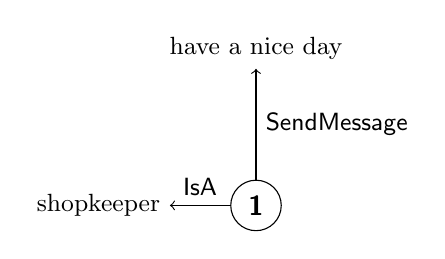
\begin{tikzpicture}[->, node distance=2cm,main node/.style={circle, draw, font=\sffamily\bfseries}]
        \tikzstyle{every node}=[font=\small]
        
          \node[main node] (1) [] {1};
          \node[] (2) [left of=1] {shopkeeper};
          \node[] (3) [above of=1]{have a nice day};
          
        
          \path[every node/.style={font=\sffamily\small}]
            (1) edge node [above] {IsA} (2)
            	edge node [right] {SendMessage} (3);
            	
        \end{tikzpicture}
        \caption{Hub for the 'shopkeeper' persona}
    \end{subfigure}%
    ~ 
    \begin{subfigure}[t]{0.45\textwidth}
        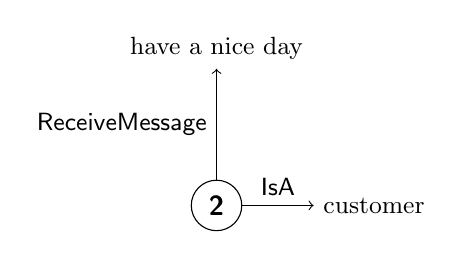
\begin{tikzpicture}[->, node distance=2cm,main node/.style={circle, draw, font=\sffamily\bfseries}]
        \tikzstyle{every node}=[font=\small]
        
          \node[main node] (1) [] {2};
          \node[] (2) [right of=1] {customer};
          \node[] (3) [above of=1]{have a nice day};
          
          
        
          \path[every node/.style={font=\sffamily\small}]
            (1) edge node [above] {IsA} (2)
            	edge node [left] {ReceiveMessage} (3);
            	
        \end{tikzpicture}
        \caption{Hub for 'customer' persona}
    \end{subfigure}
    \caption{Persona hubs diagram for shopkeeper example}
    \label{fig:shopkeeper-hubs}
\end{figure*}

\begin{figure*}[t!]
    \centering
    \begin{subfigure}[t]{0.45\textwidth}
        \centering
        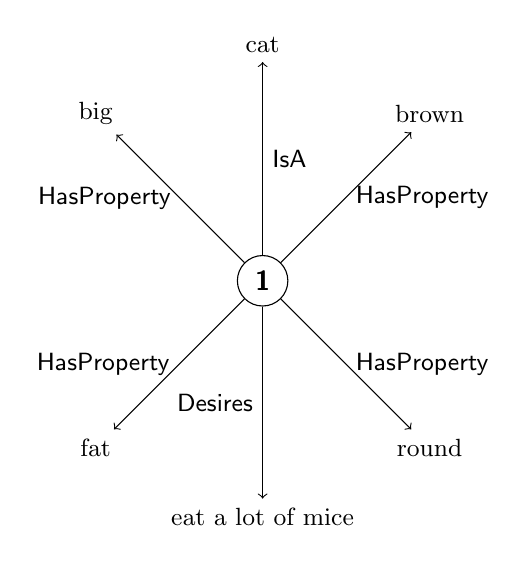
\begin{tikzpicture}[->, node distance=3cm,main node/.style={circle, draw, font=\sffamily\bfseries}]
        \tikzstyle{every node}=[font=\small]
        
          \node[main node] (1) [] {1};
          \node[] (2) [above of=1] {cat};
          \node[] (3) [above left of=1]{big};
          \node[] (4) [above right of=1] {brown};
          \node[] (5) [below right of=1] {round};
          \node[] (6) [below left of=1] {fat};
          \node[] (7) [below of=1] {eat a lot of mice};
          
        
          \path[every node/.style={font=\sffamily\small}]
            (1) edge node [right] {IsA} (2)
            	edge node [left] {HasProperty} (3)
            	edge node [right] {HasProperty} (4)
            	edge node [right] {HasProperty} (5)
            	edge node [left] {HasProperty} (6)
            	edge node [left] {Desires} (7);
            	
        \end{tikzpicture}
        \caption{Hub for the 'cat' persona}
    \end{subfigure}%
    ~ 
    \begin{subfigure}[t]{0.45\textwidth}
        \centering
        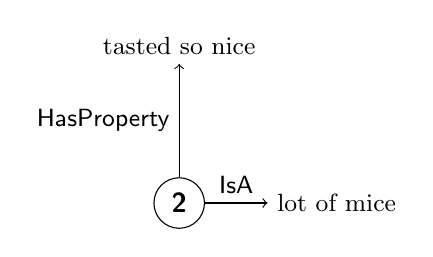
\begin{tikzpicture}[->, node distance=2cm,main node/.style={circle, draw, font=\sffamily\bfseries}]
        \tikzstyle{every node}=[font=\small]
        
          \node[main node] (1) [] {2};
          \node[] (2) [right of=1] {lot of mice};
          \node[] (3) [above of=1]{tasted so nice};
          
          
          \path[every node/.style={font=\sffamily\small}]
            (1) edge node [above] {IsA} (2)
            	edge node [left] {HasProperty} (3);
            	
        \end{tikzpicture}
        \caption{Hub for the 'lot of mice' persona}
    \end{subfigure}
    \caption{Persona hubs diagram for cat poem example}
    \label{fig:cat-hubs}
\end{figure*}


\begin{figure*}[t!]
    \centering
    \begin{subfigure}[t]{0.45\textwidth}
            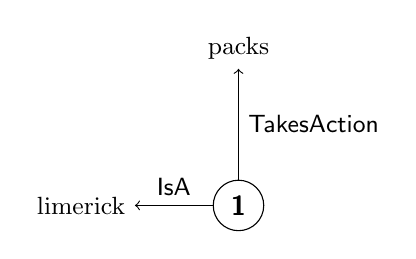
\begin{tikzpicture}[->, node distance=2cm,main node/.style={circle, draw, font=\sffamily\bfseries}]
            \tikzstyle{every node}=[font=\small]
            
              \node[main node] (1) [] {1};
              \node[] (2) [left of=1] {limerick};
              \node[] (3) [above of=1]{packs};
              
            
              \path[every node/.style={font=\sffamily\small}]
                (1) edge node [above] {IsA} (2)
                	edge node [right] {TakesAction} (3);
                	
            \end{tikzpicture}
            \caption{Hub for the 'limerick' persona}
        \end{subfigure}%
        ~ 
        \begin{subfigure}[t]{0.45\textwidth}
            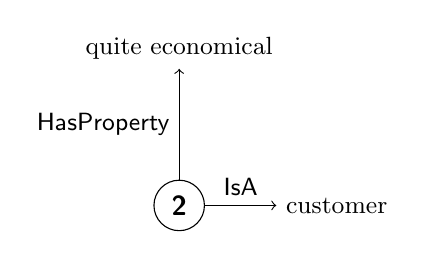
\begin{tikzpicture}[->, node distance=2cm,main node/.style={circle, draw, font=\sffamily\bfseries}]
            \tikzstyle{every node}=[font=\small]
            
              \node[main node] (1) [] {2};
              \node[] (2) [right of=1] {customer};
              \node[] (3) [above of=1]{quite economical};
              
              
              \path[every node/.style={font=\sffamily\small}]
                (1) edge node [above] {IsA} (2)
                	edge node [left] {HasProperty} (3);
                	
            \end{tikzpicture}
            \caption{Hub for 'space' persona}
        \end{subfigure}
    \begin{subfigure}[t]{0.45\textwidth}
                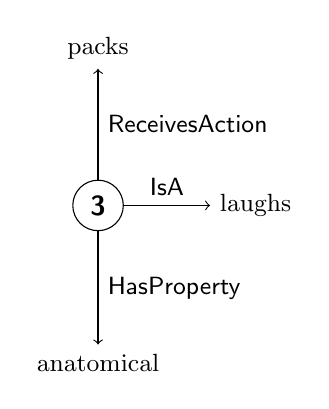
\begin{tikzpicture}[->, node distance=2cm,main node/.style={circle, draw, font=\sffamily\bfseries}]
                \tikzstyle{every node}=[font=\small]
                
                  \node[main node] (1) [] {3};
                  \node[] (2) [right of=1] {laughs};
                  \node[] (3) [above of=1]{packs};
                  \node[] (4) [below of=1]{anatomical};
                  
                
                  \path[every node/.style={font=\sffamily\small}]
                    (1) edge node [above] {IsA} (2)
                       	edge node [right] {ReceivesAction} (3)
                       	edge node [right] {HasProperty} (4);
                       	
                \end{tikzpicture}
                \caption{Hub for the 'laughs' persona}
            \end{subfigure}%
            ~ 
            \begin{subfigure}[t]{0.45\textwidth}
                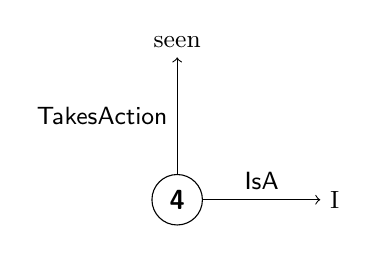
\begin{tikzpicture}[->, node distance=2cm,main node/.style={circle, draw, font=\sffamily\bfseries}]
                \tikzstyle{every node}=[font=\small]
                
                  \node[main node] (1) [] {4};
                  \node[] (2) [right of=1] {I};
                  \node[] (3) [above of=1]{seen};
                  
                  
                  \path[every node/.style={font=\sffamily\small}]
                    (1) edge node [above] {IsA} (2)
                       	edge node [left] {TakesAction} (3);
                       	
                \end{tikzpicture}
                \caption{Hub for 'I' persona}
            \end{subfigure}
    \begin{subfigure}[t]{0.45\textwidth}
            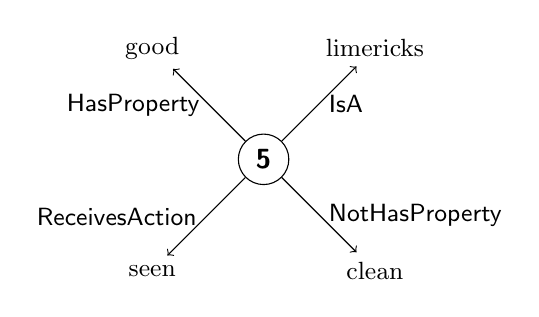
\begin{tikzpicture}[->, node distance=2cm,main node/.style={circle, draw, font=\sffamily\bfseries}]
            \tikzstyle{every node}=[font=\small]
            
              \node[main node] (1) [] {5};
              \node[] (2) [above right of=1] {limericks};
              \node[] (3) [above left of=1]{good};
              \node[] (4) [below right of=1]{clean};
              \node[] (5) [below left of=1]{seen};
              
            
              \path[every node/.style={font=\sffamily\small}]
                (1) edge node [right] {IsA} (2)
                    edge node [left] {HasProperty} (3)
                    edge node [right] {NotHasProperty} (4)
                    edge node [left] {ReceivesAction} (5);
                         	
            \end{tikzpicture}
            \caption{Hub for the persona represented by the first occurrence of 'ones'}
        \end{subfigure}%
        ~ 
        \begin{subfigure}[t]{0.45\textwidth}
            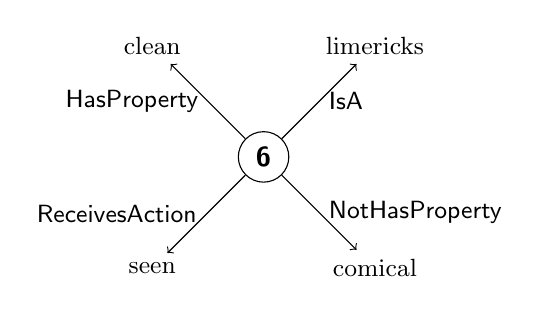
\begin{tikzpicture}[->, node distance=2cm,main node/.style={circle, draw, font=\sffamily\bfseries}]
            \tikzstyle{every node}=[font=\small]
            
              \node[main node] (1) [] {6};
	          \node[] (2) [above right of=1] {limericks};
	          \node[] (3) [above left of=1]{clean};
	          \node[] (4) [below right of=1]{comical};
	          \node[] (5) [below left of=1]{seen};
	            
	          
	          \path[every node/.style={font=\sffamily\small}]
	            (1) edge node [right] {IsA} (2)
	                edge node [left] {HasProperty} (3)
	                edge node [right] {NotHasProperty} (4)
	                edge node [left] {ReceivesAction} (5);
                         	
            \end{tikzpicture}
            \caption{Hub for the persona represented by the second occurrence of 'ones'}
        \end{subfigure}
    \caption{Persona hubs diagram for limerick example}
    \label{fig:limerick-hubs}
\end{figure*}

This will help guide the generation phase because we will know the \textit{number of persona} typical for a collection of poems, the \textit{number and type of relations} associated with \textit{each} persona, as well as allow us to find commonalities in the types of persona themselves.

To reach the desired representation, we execute Algorithm BLAH:

1 for each sentence in the poem:\\
2   get the dependency relations and frame-semantic parse\\
3	collapse loose leaves of the dependency relations\\
4	find and create possible persona objects\\
5	find candidate semantic relations from the frame-semantic parse\\
6	for each character object:\\
7		get all associated dependency relations\\
8		for each associated dependency relation:\\
9			if the dependent is involved in a candidate relation from the frame-semantic parse:\\
10				bind the relation to the current character object and continue\\
11			else:\\
12				use the heuristics for dependency relations to find possible semantic relations\\
13				bind any that are found to the current character object and continue\\
				
We will describe each step in detail.

\subsubsection{Obtaining the Semantic Dependency Relations and Frame-Semantic Parse from Noah's ARK}

We leave the frame-semantic parse from SEMAFOR in its original JSON format because we only need to access this data once when finding the candidate relations on line 5 of Algorithm BLAH. We parse the CoNLL data format of the dependencies into a dictionary shown in Table \ref{tab:DepDict} for easy access and processing downstream.

\begin{table}
\centering
    \begin{tabular}{|l|l|l|l|l|l|}
    \hline
    ID & FORM   & CPOSTAG & POSTAG & HEAD & DEPREL \\ \hline
    1  & There  & EX      & EX     & 3    & expl   \\
    2  & once   & RB      & RB     & 3    & advmod \\
    3  & was    & VB      & VBD    & 0    & null   \\
    4  & a      & DT      & DT     & 7    & det    \\
    5  & big    & JJ      & JJ     & 7    & amod   \\
    6  & brown  & JJ      & JJ     & 7    & amod   \\
    7  & cat    & NN      & NN     & 3    & nsubj  \\
    8  & who    & WP      & WP     & 9    & nsubj  \\
    9  & liked. & VB      & VBD    & 7    & rcmod  \\
    10 & to     & TO      & TO     & 11   & aux    \\
    11 & eat    & VB      & VB     & 9    & xcomp  \\
    12 & a      & DT      & DT     & 13   & det    \\
    13 & lot    & NN      & NN     & 11   & dobj   \\
    14 & of     & IN      & IN     & 13   & prep   \\
    15 & mice   & NN      & NNS    & 14   & pobj   \\
    16 & .      & .       & .      & 3    & punct  \\ \hline
    \end{tabular}
\caption{The dependencies dictionary data structure for the first sentence of the cat poem.}
\label{tab:DepDict}
\end{table}

\subsubsection{Collapsing Loose Leaves of Dependency Relations}
\label{sec:collapse}

In a lot of cases, the persona or relation that we look for are represented by phrases, not just a words. For example in Figure \ref{fig:cat-deps1} the character should be \textit{'a lot of mice'} rather than just the noun \textit{'mice'}. In fact if we skipped this step of the algorithm, we would get two characters - \textit{'lot'} and \textit{'mice'} - which is obviously wrong.

\begin{figure}[h!]
\centering
\includegraphics[width=140mm]{cat-deps1}
\caption{TurboParser Semantic Dependency parse for the first sentence of the cat poem.}
\label{fig:cat-deps1}
\end{figure}

\begin{figure}[h!]
\centering
\includegraphics[width=140mm]{cat-deps2}
\caption{TurboParser Semantic Dependency parse for the second sentence of the cat poem.}
\label{fig:cat-deps2}
\end{figure}

Another example is the phrase \textit{'tasted so nice'} as in Figure \ref{fig:cat-deps2}. If we did not collapse the tree, we would have that \textit{'they'} can be described as \textit{'nice'} and took the action of \textit{'taste'}, both of which are wrong again.

To solve this, we merge leaves of the tree together if the dependency is \textit{'collapsable'} as per a set of conditions listed in the Appendix, section \ref{sec:collapsable}.

By default, the parent of the dependency keeps all its attributes unchanged except for merging its form with that of the leaf, e.g. \textit{'of'} and \textit{'mice'} becomes \textit{'of mice'}. However, there are some cases where we wish to retain the part-of-speech (POS) tag of the leaf and overwrite the parent's POS tag:

\begin{itemize}
\item{If the leaf is an adjective, the parent is a verb and the dependency relation is \textit{dep} then we retain the adjective POS tag. These conditions usually imply a \textit{linking verb}, generally used to describe a property; not an action. For example, \textit{tasted so nice} is an adjectival phrase despite the use of a verb.}
\item{Collapsing an \textit{acomp} dependency relation should also retain the child POS tag because it too is evidence of a linking verb.}
\item{The \textit{pobj} and \textit{prep} dependency relations are evidence of prepositions, which often link words together that lose meaning when separated. For example, \textit{'of mice'} should retain the 'NNS' POS tag of \textit{'mice'} rather than keep the 'PRP' POS tag of \textit{'of'}.}
\end{itemize}

Then we follow Algorithm BLAH:\\
1 Get a list of all the leaves in the graph.\\
2 For each leaf in the reverse of this list:\\
3	If the dependency relation of this leaf (i.e. from its parent to it) is collapsable:\\
4		Get the parent\\
5		Merge the form of the parent and the leaf\\
6		If necessary, the parent retains the part-of-speech tag of the leaf\\
7		The leaf is destroyed and the parent becomes the leaf.\\
8		Loop back to line 3.\\

Figure \ref{fig:cat-deps1-collapsed} shows a dry run of this algorithm on the first line of the cat poem as shown in Figure \ref{fig:cat-deps1}.

\begin{figure}[h!]
\centering
\begin{subfigure}[t]{0.9\textwidth}
	\centering
    \includegraphics[width=140mm]{cat-deps1-collapsed-a}
    \caption{Identify all of the leaves}
\end{subfigure}
\begin{subfigure}[t]{0.9\textwidth}
	\centering
    \includegraphics[width=140mm]{cat-deps1-collapsed-b}
    \caption{Start from the rightmost leaf, \textit{'mice'} (ignore punctuation). Dependency \textit{'pobj'} is collapsable and we inherit the child POS tag.}
\end{subfigure}
\begin{subfigure}[t]{0.9\textwidth}
	\centering
    \includegraphics[width=140mm]{cat-deps1-collapsed-c}
    \caption{Because we collapsed a leaf in the previous step and it remained a leaf, we see if we can collapse the same leaf further. Dependency \textit{'prep'} is collapsable and we inherit the child POS tag once again.}
\end{subfigure}
\begin{subfigure}[t]{0.9\textwidth}
	\centering
    \includegraphics[width=140mm]{cat-deps1-collapsed-d}
    \caption{The leaf we collapsed is now a parent so we move left to the next leaf \textit{'a'}. Dependency \textit{'det'} is collapsable and we retain the parent POS tag this time.}
\end{subfigure}
\begin{subfigure}[t]{0.9\textwidth}
	\centering
    \includegraphics[width=140mm]{cat-deps1-collapsed-e}
    \caption{We have a leaf again, but we cannot collapse any further. We move on to the next leaf, \textit{'to'}. Dependency \textit{'aux'} is collapsable and we retain the parent POS tag.}
\end{subfigure}
\begin{subfigure}[t]{0.9\textwidth}
	\centering
    \includegraphics[width=140mm]{cat-deps1-collapsed-f}
    \caption{Move on to next leaves. Dependencies \textit{'nsubj'} and \textit{'amod'} are not collapsable, but \textit{'det'} is so we collapse leaf \textit{'a'} with its parent \textit{'cat'}.}
\end{subfigure}
\begin{subfigure}[t]{0.9\textwidth}
	\centering
    \includegraphics[width=140mm]{cat-deps1-collapsed-g}
    \caption{Dependency \textit{'advmod'} is collapsable and \textit{'expl'} is not. Collapse accordingly and finish.}
    \label{fig:cat-deps1-collapsed-g}
\end{subfigure}
\caption{Execution of Algorithm BLAH on the first half of the cat poem example.}
\label{fig:cat-deps1-collapsed}
\end{figure}

The final diagrams of the collapsed dependencies for the full cat poem example can be seen in \ref{fig:cat-collapsed}

\begin{figure}[H]
\centering
\begin{subfigure}[t]{0.9\textwidth}
	\centering
    \includegraphics[width=140mm]{cat-deps1-collapsed-g}
    \caption{First sentence.}
    \label{fig:cat-deps1-collapsed-g-final}
\end{subfigure}
\begin{subfigure}[t]{0.9\textwidth}
	\centering
    \includegraphics[width=140mm]{cat-deps2-collapsed}
    \caption{Second sentence.}
    \label{fig:cat-deps2-collapsed}
\end{subfigure}
\caption{Final collapsed dependency diagrams for full cat poem example.}
\label{fig:cat-collapsed}
\end{figure}

\subsubsection{Finding and Creating Characters}
\label{sec:characters} 

A naive method for finding persona would be to simply extract nouns and pronouns. This would actually be sufficient for a basic level of analysis, but this does not account for anaphora and presuppositions (see Section \ref{sec:arback}). Notice that in the second half of the cat poem, the pronoun \textit{'he'} is used to refer to the 'cat' persona and \textit{'they'} to the 'a lot of mice' persona.

I will not be using any out-of-the box anaphora resolution tools like the ones mentioned in \ref{sec:arback}. Instead, I will present a new potential solution in section \ref{sec:ar}.

Part of the solution requires some basic semantic information about the persona as a prerequisite. We would like to determine whether the phrase representing the character:

\begin{enumerate}
\item{is plural or singular.}
\item{is male, female, neutral or unknown.}
\item{is a living object, an inanimate physical object or a non-object.}
\end{enumerate}

Determining the first point is the most straightforward:
\begin{itemize}
\item{if it is a noun and the POS tag ends in an 'S', it is plural (see \textit{'mice'} tag in \ref{fig:cat-deps1}).}
\item{if it is a pronoun, check for membership in a manually built list of plural pronouns (e.g. 'they', 'them').}
\end{itemize}

The pronoun case for the second point is similar; we check for membership in the manually built list of male pronouns (e.g. 'he', 'him') and the separate list of female pronouns (e.g. 'she', 'her'). 

The noun case is trickier. First we need to find the \textit{synset} of the noun. Once we have this, we can use the \textit{hypernym} relationships between synsets. Finally, we can check for whether a noun is male or female by looking for the existence of particular synsets that imply a gender. For example, the \textit{'female'} synset would be an inherited hypernym of the synset \textit{'cow'}. Therefore we know that cows are female. Similarly, \textit{'maharaja'} has the hypernym \textit{'prince'}, which we know to be male.

We can extend this practice to the final point of determining the animation of the character by checking if the \textit{'living thing'} and \textit{'physical object'} synsets are inherited hypernyms of the synset of the noun concerned.


\subsubsection{Extracting Candidate Relations from the Frame-Semantic Parse}
\label{sec:candidate}

Using the map between FrameNet frames and semantic relations mentioned in section \ref{sec:sema}, we can carry out Algorithm BLAH.

1 for each frame found in the frame-semantic parse:\\
2	look up the target of the frame in the map\\
3	if it can help build a relation:	\\
4		retrieve the frame elements\\
5		match the frame elements with the corresponding text from the poem\\
6			if we cannot find all the elements we are looking for, we leave it blank\\
7		add mapping from the text of the target to the newly built relation so we can find it later\\
	
Figure \ref{fig:cat1-fn-cn} show a dry run of this algorithm using the first half of the cat poem in Figure \ref{fig:cat}.

\begin{figure}[H]
\centering
\begin{subfigure}[t]{0.9\textwidth}
	\centering
    \includegraphics[width=140mm]{cat1-fn-cn-a}
    \caption{Get all the frames found by the frame-semantic parse}
\end{subfigure}
\begin{subfigure}[t]{0.9\textwidth}
	\centering
    \includegraphics[width=140mm]{cat1-fn-cn-b}
    \caption{The only one that we can convert to a relation is the Experiencer\_Focus frame}
\end{subfigure}
\begin{subfigure}[t]{0.9\textwidth}
	\centering
    \includegraphics[width=140mm]{cat1-fn-cn-c}
    \caption{Retrieve the frame elements with an anchor on the target text, \textit{'liked'}}
\end{subfigure}
\begin{subfigure}[t]{0.9\textwidth}
	\centering
    \includegraphics[width=140mm]{cat1-fn-cn-d}
    \caption{Create the corresponding relation and map it to the target}
\end{subfigure}
\caption{Execution of Algorithm BLAH on the first half of the cat poem example.}
\label{fig:cat1-fn-cn}
\end{figure}

No frames could be converted into relations for the second half of the cat poem example.

\subsubsection{Obtaining the Associated Dependency Relations for each Persona}

This step breaks up the semantic dependency tree and flattens it into the character-centric hubs like the ones in Figure \ref{fig:cat-hubs}. We start from Figure \ref{fig:cat-deps1-collapsed-g}.

First, we want to identify the persona in the dependency tree. All of the relations going out from it are naturally related dependencies of the persona, so they get added to the hub.

The single relation coming into this character is also a related dependency. We reverse the direction of the branch and add it to the hub. The hub so far is more like a spider diagram, as shown in Figure \ref{fig:cat-in-out-deps}.

\begin{figure}[H]
    \centering
    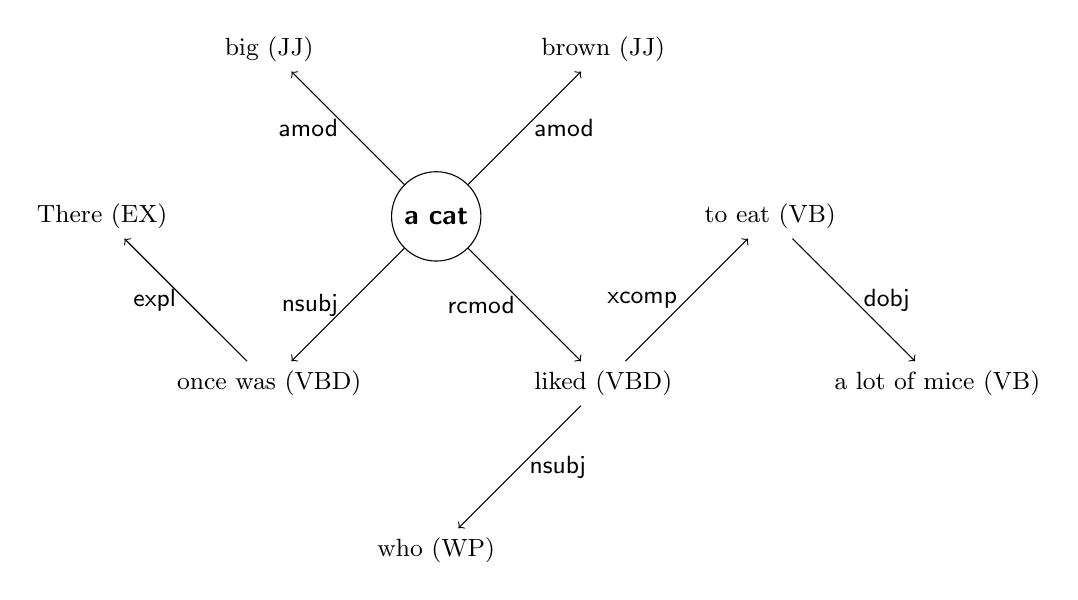
\begin{tikzpicture}[->, node distance=3cm,main node/.style={circle, draw, font=\sffamily\bfseries}]
    \tikzstyle{every node}=[font=\small]
    
      \node[main node] (1) [] {a cat};
      \node[] (3) [above left of=1]{big (JJ)};
      \node[] (4) [above right of=1] {brown (JJ)};
      \node[] (5) [below right of=1] {liked (VBD)};
      \node[] (6) [below left of=5] {who (WP)};
      \node[] (7) [above right of=5] {to eat (VB)};
      \node[] (8) [below right of=7] {a lot of mice (VB)};
      \node[] (9) [below left of=1] {once was (VBD)};
      \node[] (10) [above left of=9] {There (EX)};
      
    
      \path[every node/.style={font=\sffamily\small}]
        (1) edge node [left] {amod} (3)
           	edge node [right] {amod} (4)
           	edge node [left] {rcmod} (5)
           	edge node [left] {nsubj} (9)
        (5) edge node [right] {nsubj} (6)
            edge node [left] {xcomp} (7)
        (7) edge node [right] {dobj} (8)
        (9) edge node [left] {expl} (10);
          
    \end{tikzpicture}
    \caption{Initial dependency hub for the 'cat' persona.}
    \label{fig:cat-in-out-deps}
\end{figure}%

Now we have a tree with the character as the root. The next step is to flatten it so that all nodes are directly related to the character. We do this by recursively converting all the grandchildren of the character root node to a direct child node until there are no more grandchildren. This is shown in Figure \ref{fig:first-hubs}.

We repeat this process for each persona starting from the leftmost character in the sentence. The persona hubs for the second half of the poem is shown in Figure \ref{fig:second-hubs}.

\begin{figure}[H]
\centering
\begin{subfigure}[t]{0.9\textwidth}
	\centering
    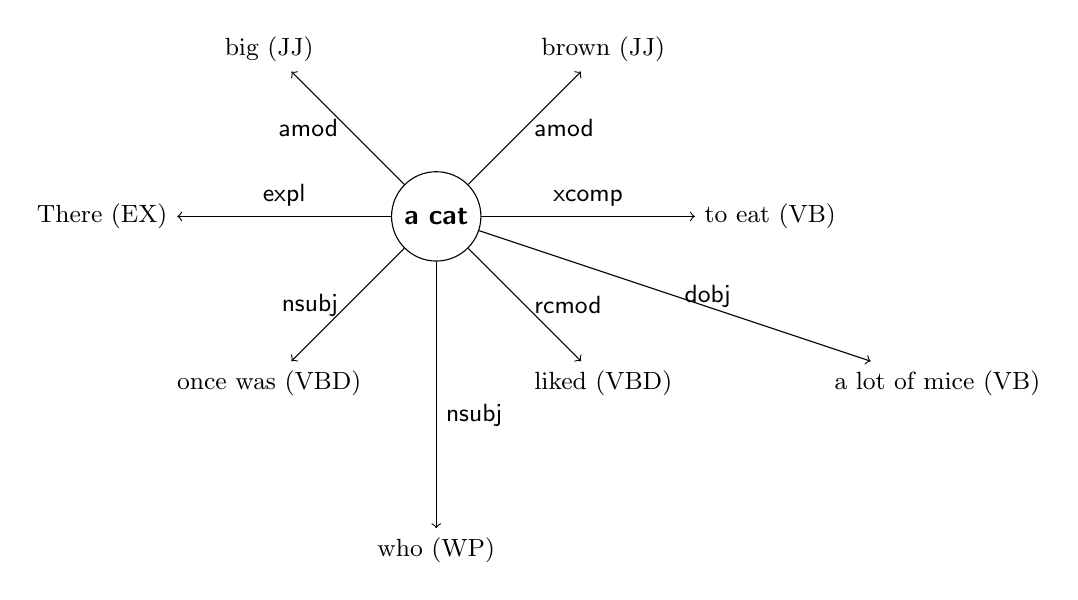
\begin{tikzpicture}[->, node distance=3cm,main node/.style={circle, draw, font=\sffamily\bfseries}]
        \tikzstyle{every node}=[font=\small]
        
          \node[main node] (1) [] {a cat};
          \node[] (3) [above left of=1]{big (JJ)};
          \node[] (4) [above right of=1] {brown (JJ)};
          \node[] (5) [below right of=1] {liked (VBD)};
          \node[] (6) [below left of=5] {who (WP)};
          \node[] (7) [above right of=5] {to eat (VB)};
          \node[] (8) [below right of=7] {a lot of mice (VB)};
          \node[] (9) [below left of=1] {once was (VBD)};
          \node[] (10) [above left of=9] {There (EX)};
          
        
          \path[every node/.style={font=\sffamily\small}]
            (1) edge node [left] {amod} (3)
               	edge node [right] {amod} (4)
               	edge node [right] {rcmod} (5)
               	edge node [left] {nsubj} (9)
                edge node [below right] {nsubj} (6)
                edge node [above] {xcomp} (7)
                edge node [right] {dobj} (8)
                edge node [above] {expl} (10);
              
        \end{tikzpicture}
    \caption{Persona: 'cat'}
\end{subfigure}
\begin{subfigure}[t]{0.9\textwidth}
	\centering
    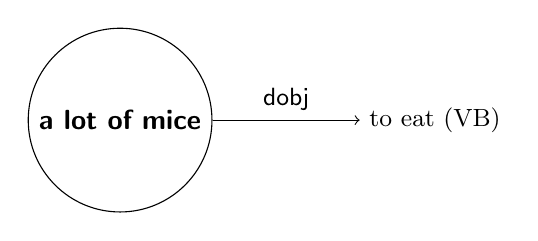
\begin{tikzpicture}[->, node distance=4cm,main node/.style={circle, draw, font=\sffamily\bfseries}]
        \tikzstyle{every node}=[font=\small]
        
          \node[main node] (1) [] {a lot of mice};
          \node[] (2) [right of=1]{to eat (VB)};
          
        
          \path[every node/.style={font=\sffamily\small}]
            (1) edge node [above] {dobj} (2);
              
        \end{tikzpicture}
    \caption{Persona: 'a lot of mice'}
\end{subfigure}
\caption{All persona hubs for the first sentence of the cat example.}
\label{fig:first-hubs}
\end{figure}

\begin{figure}[H]
\centering
\begin{subfigure}[t]{0.9\textwidth}
	\centering
    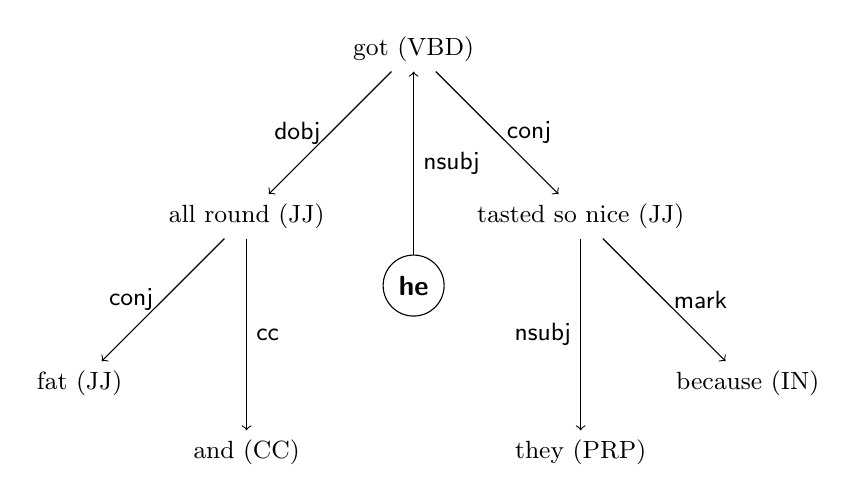
\begin{tikzpicture}[->, node distance=3cm,main node/.style={circle, draw, font=\sffamily\bfseries}]
        \tikzstyle{every node}=[font=\small]
        
          \node[main node] (1) [] {he};
          \node[] (2) [above of=1]{got (VBD)};
          \node[] (3) [below right of=2]{tasted so nice (JJ)};
          \node[] (4) [below of=3]{they (PRP)};
          \node[] (5) [below right of=3]{because (IN)};
          \node[] (6) [below left of=2]{all round (JJ)};
          \node[] (7) [below of=6]{and (CC)};
          \node[] (8) [below left of=6]{fat (JJ)};
          
        
          \path[every node/.style={font=\sffamily\small}]
            (1) edge node [right] {nsubj} (2)
            (2) edge node [right] {conj} (3)
                edge node [left] {dobj} (6)
            (3) edge node [left] {nsubj} (4)
                edge node [right] {mark} (5)
            (6) edge node [right] {cc} (7)
                edge node [left] {conj} (8);
              
        \end{tikzpicture}
    \caption{Persona: 'he' before flattening.}
\end{subfigure}
\begin{subfigure}[t]{0.9\textwidth}
	\centering
    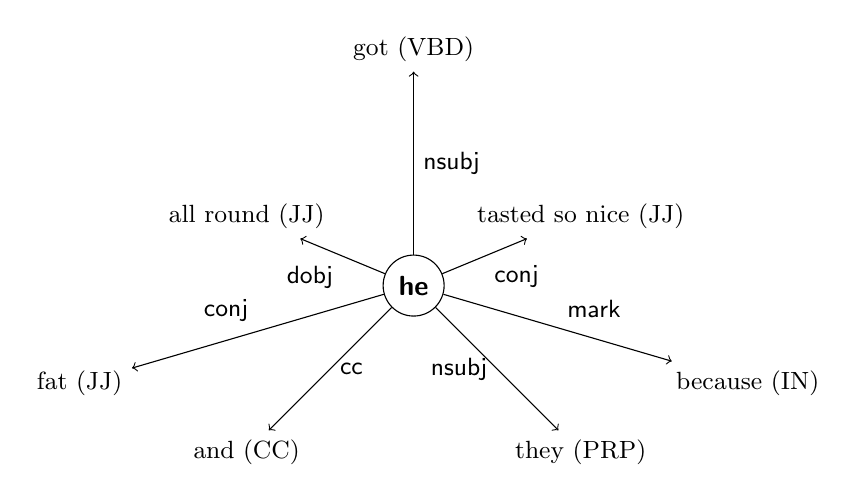
\begin{tikzpicture}[->, node distance=3cm,main node/.style={circle, draw, font=\sffamily\bfseries}]
        \tikzstyle{every node}=[font=\small]
        
          \node[main node] (1) [] {he};
          \node[] (2) [above of=1]{got (VBD)};
          \node[] (3) [below right of=2]{tasted so nice (JJ)};
          \node[] (4) [below of=3]{they (PRP)};
          \node[] (5) [below right of=3]{because (IN)};
          \node[] (6) [below left of=2]{all round (JJ)};
          \node[] (7) [below of=6]{and (CC)};
          \node[] (8) [below left of=6]{fat (JJ)};
          
        
          \path[every node/.style={font=\sffamily\small}]
            (1) edge node [right] {nsubj} (2)
                edge node [below right] {conj} (3)
                edge node [below left] {dobj} (6)
                edge node [left] {nsubj} (4)
                edge node [above right] {mark} (5)
                edge node [right] {cc} (7)
                edge node [above left] {conj} (8);
              
        \end{tikzpicture}
    \caption{Persona: 'he' after flattening.}
\end{subfigure}
\begin{subfigure}[t]{0.45\textwidth}
	\centering
    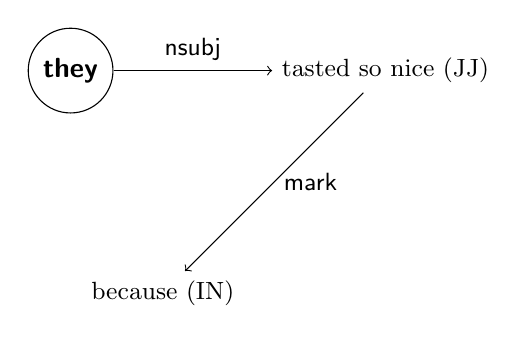
\begin{tikzpicture}[->, node distance=4cm,main node/.style={circle, draw, font=\sffamily\bfseries}]
        \tikzstyle{every node}=[font=\small]
        
          \node[main node] (1) [] {they};
          \node[] (2) [right of=1]{tasted so nice (JJ)};
          \node[] (3) [below left of=2]{because (IN)};
          
        
          \path[every node/.style={font=\sffamily\small}]
            (1) edge node [above] {nsubj} (2)
            (2) edge node [right] {mark} (3);
              
        \end{tikzpicture}
    \caption{Persona: 'they' before flattening}
\end{subfigure}
~
\begin{subfigure}[t]{0.45\textwidth}
	\centering
    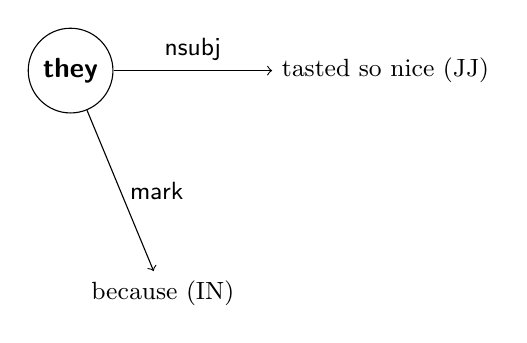
\begin{tikzpicture}[->, node distance=4cm,main node/.style={circle, draw, font=\sffamily\bfseries}]
        \tikzstyle{every node}=[font=\small]
        
          \node[main node] (1) [] {they};
          \node[] (2) [right of=1]{tasted so nice (JJ)};
          \node[] (3) [below left of=2]{because (IN)};
          
        
          \path[every node/.style={font=\sffamily\small}]
            (1) edge node [above] {nsubj} (2)
                edge node [right] {mark} (3);
              
        \end{tikzpicture}
    \caption{Persona: 'they' after flattening}
\end{subfigure}
\caption{All persona hubs for the second sentence of the cat example.}
\label{fig:second-hubs}
\end{figure}

Notice that the same \textit{mark} dependency with node \textit{[because (IN)]} is associated to both \textit{'he'} and \textit{'they'}. The \textit{[tasted so nice (JJ)]} node is also involved with both of them, although the type of dependency differs.

In most cases, we do not want either of these duplicated dependencies as it can lead to redundant relations. We will deal with this in the next step where we convert these dependencies into relations.

\subsubsection{Binding ConceptNet Relations to Characters}
	
Now that we have our hub data structure for all persona, we now need to look at each branch of each hub and decide if it can be converted into a semantic relation.

First, we check if the text of the child maps to the target of one of the candidate relations we extracted from the frame-semantic parse in section \ref{sec:candidate}. If it does, then we accept that and move on to the next child without checking the dependency relation since it is likely to be the less accurate or redundant. 

Sometimes the dependant of the relation will be blank because we could not find the right frame element as explained earlier. In this case, we just assume that this is a relation to the next persona in the list. This is a fair assumption given the limited number of persona per sentence, the probable forward reference structure of sentences and the fact that most of the relations we look to build are between persona.

If there is no candidate relation for this child, we then look at the type of the dependency between it and the persona. We use the heuristics described in section \ref{sec:turbo} to convert it into a semantic relation.

If we cannot find a relation using either of the above methods then it is unlikely that one exists, so we remove it from the hub and move on to the next child.

In all of those steps, we need to look out for negative adverbs such as 'not', 'seldom', 'rarely' etc. which we use to negate the relation found. We also need to look out for antonyms in the target word in the frame-semantic parse. For example, the \textit{Experiencer-focus} frame helps us find \textit{Desires} and \textit{NotDesires} ConceptNet relations depending on whether the target word is synonymous with 'love' or 'hate'.

To avoid the aforementioned duplication problem, we prune these hubs by working backwards through the persona (i.e. starting from the rightmost in the sentence) and removing any relations that occur in earlier persona. So in fact the \textit{'lot of mice'} persona has no relations (before anaphora resolution, see Section \ref{sec:ar}).

The duplication is mostly due to reversing the direction on incoming dependencies (heads). This pruning method works because the head of the last persona will be lower down in the dependency tree than the head of any other persona. Duplicated relations are removed such that it is solely associated to the one it was closest to in the original tree.

We can see this entire process being applied step-by-step to the 'cat' persona in our ongoing example in Figure \ref{fig:cat-bind}. The final hubs for all persona can be seen in Figure \ref{fig:all-binded}.

\begin{figure}[h!]
\centering
\begin{subfigure}[t]{0.45\textwidth}
	\centering
    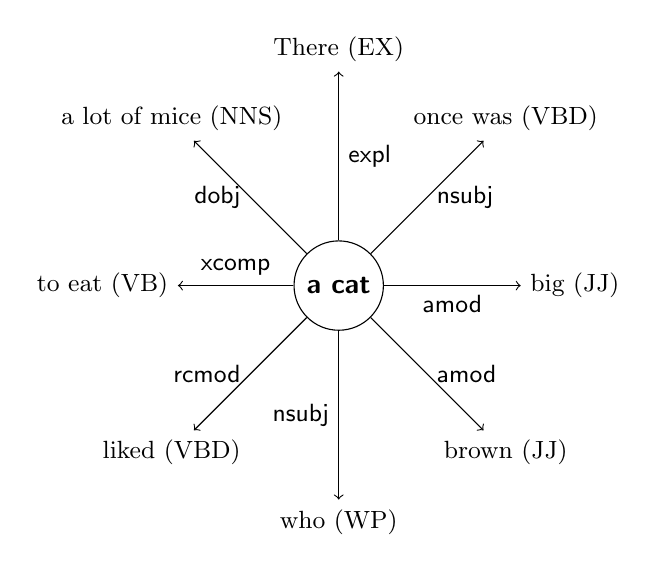
\begin{tikzpicture}[->, node distance=3cm,main node/.style={circle, draw, font=\sffamily\bfseries}]
        \tikzstyle{every node}=[font=\small]
        
          \node[main node] (1) [] {a cat};
          \node[] (3) [right of=1]{big (JJ)};
          \node[] (4) [below right of=1] {brown (JJ)};
          \node[] (5) [below left of=1] {liked (VBD)};
          \node[] (6) [below of=1] {who (WP)};
          \node[] (7) [left of=1] {to eat (VB)};
          \node[] (8) [above left of=1] {a lot of mice (NNS)};
          \node[] (9) [above right of=1] {once was (VBD)};
          \node[] (10) [above of=1] {There (EX)};
          
        
          \path[every node/.style={font=\sffamily\small}]
            (1) edge node [below] {amod} (3)
               	edge node [right] {amod} (4)
               	edge node [left] {rcmod} (5)
               	edge node [right] {nsubj} (9)
                edge node [left] {nsubj} (6)
                edge node [above] {xcomp} (7)
                edge node [left] {dobj} (8)
                edge node [right] {expl} (10);
              
        \end{tikzpicture}
    \caption{Dependency hub for the 'cat' character, rearranged such that the children appear in the order they do in the original sentence, starting from \textit{'There'} in the 12 o'clock position in a clockwise direction.}
\end{subfigure}
~
\begin{subfigure}[t]{0.45\textwidth}
	\centering
    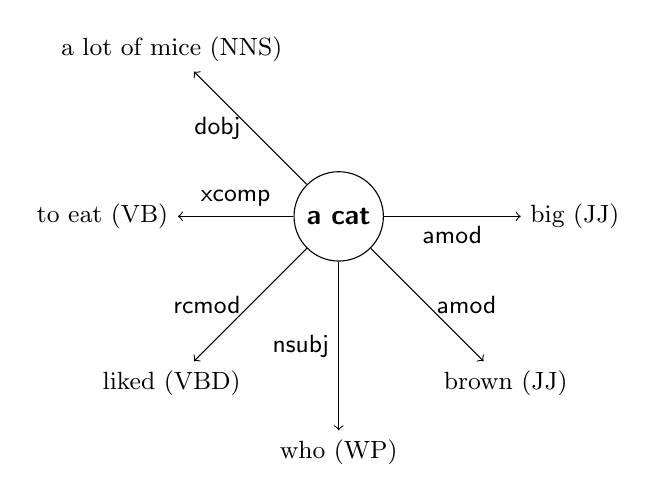
\begin{tikzpicture}[->, node distance=3cm,main node/.style={circle, draw, font=\sffamily\bfseries}]
        \tikzstyle{every node}=[font=\small]
        
          \node[main node] (1) [] {a cat};
          \node[] (3) [right of=1]{big (JJ)};
          \node[] (4) [below right of=1] {brown (JJ)};
          \node[] (5) [below left of=1] {liked (VBD)};
          \node[] (6) [below of=1] {who (WP)};
          \node[] (7) [left of=1] {to eat (VB)};
          \node[] (8) [above left of=1] {a lot of mice (NNS)};
          
        
          \path[every node/.style={font=\sffamily\small}]
            (1) edge node [below] {amod} (3)
               	edge node [right] {amod} (4)
               	edge node [left] {rcmod} (5)
                edge node [left] {nsubj} (6)
                edge node [above] {xcomp} (7)
                edge node [left] {dobj} (8);
              
        \end{tikzpicture}
    \caption{Dependency \textit{expl} does not map to any relation and the child \textit{'There (EX)'} does not map to any relation via the frame-semantic parse. It is removed. Similarly remove the \textit{'once was (VB)'} child because it is a verb but the lemma includes the verb 'be'.}
\end{subfigure}
\caption{Full binding process for the 'cat' character}
\label{fig:cat-bind}
\end{figure}

\begin{figure}[h!]
\ContinuedFloat
\centering
\begin{subfigure}[t]{0.45\textwidth}
	\centering
    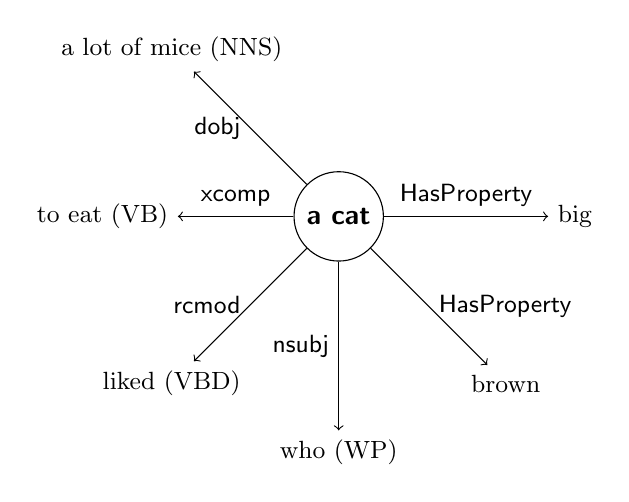
\begin{tikzpicture}[->, node distance=3cm,main node/.style={circle, draw, font=\sffamily\bfseries}]
        \tikzstyle{every node}=[font=\small]
        
          \node[main node] (1) [] {a cat};
          \node[] (3) [right of=1]{big};
          \node[] (4) [below right of=1] {brown};
          \node[] (5) [below left of=1] {liked (VBD)};
          \node[] (6) [below of=1] {who (WP)};
          \node[] (7) [left of=1] {to eat (VB)};
          \node[] (8) [above left of=1] {a lot of mice (NNS)};
          
        
          \path[every node/.style={font=\sffamily\small}]
            (1) edge node [above] {HasProperty} (3)
               	edge node [right] {HasProperty} (4)
               	edge node [left] {rcmod} (5)
                edge node [left] {nsubj} (6)
                edge node [above] {xcomp} (7)
                edge node [left] {dobj} (8);
              
        \end{tikzpicture}
    \caption{Dependency \textit{'amod'} maps directly to a HasProperty relation for both the \textit{'big (JJ)'} and \textit{'brown (JJ)'} children.}
\end{subfigure}
~
\begin{subfigure}[t]{0.45\textwidth}
	\centering
    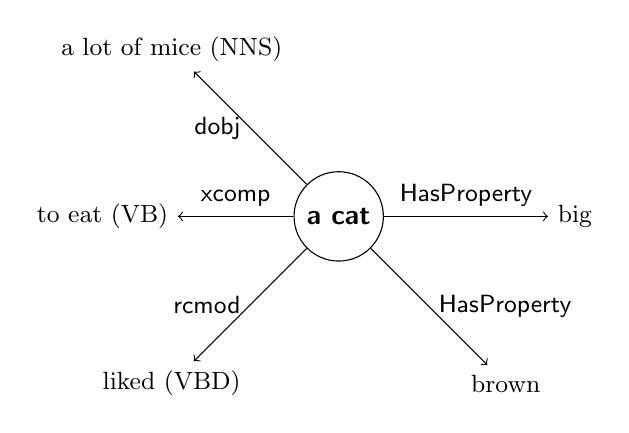
\begin{tikzpicture}[->, node distance=3cm,main node/.style={circle, draw, font=\sffamily\bfseries}]
        \tikzstyle{every node}=[font=\small]
        
          \node[main node] (1) [] {a cat};
          \node[] (3) [right of=1]{big};
          \node[] (4) [below right of=1] {brown};
          \node[] (5) [below left of=1] {liked (VBD)};
          \node[] (7) [left of=1] {to eat (VB)};
          \node[] (8) [above left of=1] {a lot of mice (NNS)};
          
        
          \path[every node/.style={font=\sffamily\small}]
            (1) edge node [above] {HasProperty} (3)
               	edge node [right] {HasProperty} (4)
               	edge node [left] {rcmod} (5)
                edge node [above] {xcomp} (7)
                edge node [left] {dobj} (8);
              
        \end{tikzpicture}
    \caption{Remove the \textit{'who (WP)'} child because it has a POS tag starting with W so the \textit{'nsubj'} relation does not matter.}
\end{subfigure}
~
\begin{subfigure}[t]{0.45\textwidth}
	\centering
    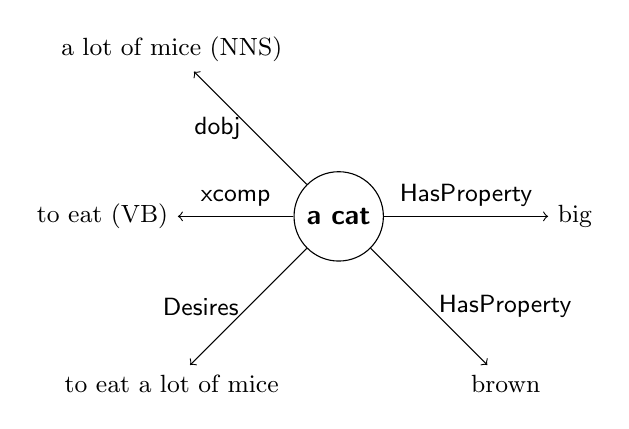
\begin{tikzpicture}[->, node distance=3cm,main node/.style={circle, draw, font=\sffamily\bfseries}]
        \tikzstyle{every node}=[font=\small]
        
          \node[main node] (1) [] {a cat};
          \node[] (3) [right of=1]{big};
          \node[] (4) [below right of=1] {brown};
          \node[] (5) [below left of=1] {to eat a lot of mice};
          \node[] (7) [left of=1] {to eat (VB)};
          \node[] (8) [above left of=1] {a lot of mice (NNS)};
          
        
          \path[every node/.style={font=\sffamily\small}]
            (1) edge node [above] {HasProperty} (3)
               	edge node [right] {HasProperty} (4)
               	edge node [left] {Desires} (5)
                edge node [above] {xcomp} (7)
                edge node [left] {dobj} (8);
              
        \end{tikzpicture}
    \caption{In this case, \textit{'liked (VBD)'} is a target mapped to a relation found from the frame-semantic parse. It gets replaced by this relation with no further consideration.}
\end{subfigure}
~
\begin{subfigure}[t]{0.45\textwidth}
	\centering
    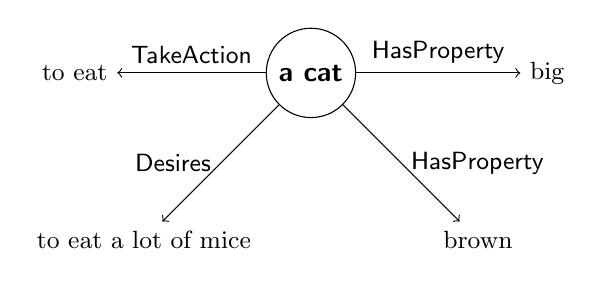
\begin{tikzpicture}[->, node distance=3cm,main node/.style={circle, draw, font=\sffamily\bfseries}]
        \tikzstyle{every node}=[font=\small]
        
          \node[main node] (1) [] {a cat};
          \node[] (3) [right of=1]{big};
          \node[] (4) [below right of=1] {brown};
          \node[] (5) [below left of=1] {to eat a lot of mice};
          \node[] (7) [left of=1] {to eat};
          
        
          \path[every node/.style={font=\sffamily\small}]
            (1) edge node [above] {HasProperty} (3)
               	edge node [right] {HasProperty} (4)
               	edge node [left] {Desires} (5)
                edge node [above] {TakeAction} (7);
              
        \end{tikzpicture}
    \caption{The final \textit{'a lot of mice (NNS)'} child is not a verb so the \textit{'dobj'} relation has no effect.}
\end{subfigure}
\caption{Full binding process for the 'cat' character}
%\label{fig:cat-bind}
\end{figure}

\begin{figure}[h!]
\centering
\begin{subfigure}[t]{0.9\textwidth}
	\centering
    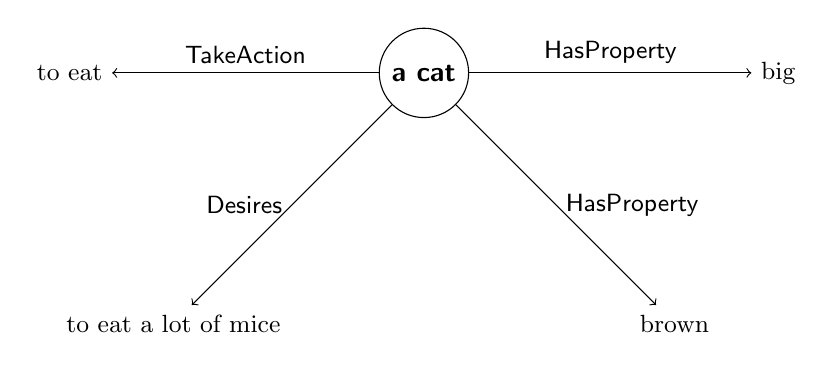
\begin{tikzpicture}[->, node distance=4.5cm,main node/.style={circle, draw, font=\sffamily\bfseries}]
        \tikzstyle{every node}=[font=\small]
        
          \node[main node] (1) [] {a cat};
          \node[] (3) [right of=1]{big};
          \node[] (4) [below right of=1] {brown};
          \node[] (5) [below left of=1] {to eat a lot of mice};
          \node[] (7) [left of=1] {to eat};
          
        
          \path[every node/.style={font=\sffamily\small}]
            (1) edge node [above] {HasProperty} (3)
               	edge node [right] {HasProperty} (4)
               	edge node [left] {Desires} (5)
                edge node [above] {TakeAction} (7);
              
        \end{tikzpicture}
    \caption{Bindings for 'cat' persona.}
\end{subfigure}
\begin{subfigure}[t]{0.9\textwidth}
	\centering
    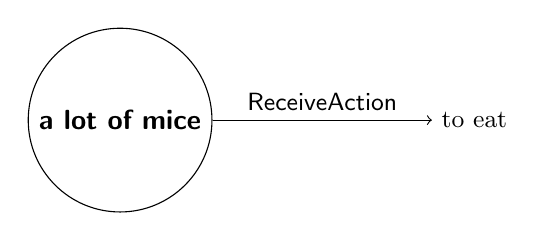
\begin{tikzpicture}[->, node distance=4.5cm,main node/.style={circle, draw, font=\sffamily\bfseries}]
        \tikzstyle{every node}=[font=\small]
        
          \node[main node] (1) [] {a lot of mice};
          \node[] (2) [right of=1]{to eat};
          
          \path[every node/.style={font=\sffamily\small}]
            (1) edge node [above] {ReceiveAction} (2);
              
        \end{tikzpicture}
    \caption{Bindings for 'lot of mice' persona.}
\end{subfigure}
\begin{subfigure}[t]{0.9\textwidth}
	\centering
    \begin{tikzpicture}[->, node distance=4.5cm,main node/.style={circle, draw, font=\sffamily\bfseries}]
        \tikzstyle{every node}=[font=\small]
        
          \node[main node] (1) [] {he};
          \node[] (2) [right of=1]{got (VBD)};
          \node[] (6) [below left of=1]{all round};
          \node[] (8) [above left of=1]{fat};
          
        
          \path[every node/.style={font=\sffamily\small}]
            (1) edge node [above] {TakeAction} (2)
                edge node [left] {HasProperty} (6)
                edge node [left] {HasProperty} (8);
              
        \end{tikzpicture}
    \caption{Bindings for 'he' persona. Notice \textit{'tasted so nice (JJ)'} was removed from here because of duplication with \textit{'they'} persona below. We get one anomaly with \textit{'got'} because we were unable to distinguish between definitions of 'became' and 'retrieved'.}
\end{subfigure}
\begin{subfigure}[t]{0.9\textwidth}
	\centering
    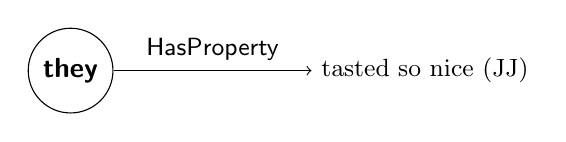
\begin{tikzpicture}[->, node distance=4.5cm,main node/.style={circle, draw, font=\sffamily\bfseries}]
        \tikzstyle{every node}=[font=\small]
        
          \node[main node] (1) [] {they};
          \node[] (2) [right of=1]{tasted so nice (JJ)};
          
        
          \path[every node/.style={font=\sffamily\small}]
            (1) edge node [above] {HasProperty} (2);
              
        \end{tikzpicture}
    \caption{Bindings for 'they' persona.}
\end{subfigure}
\caption{Complete bindings for all persona}
\label{fig:all-binded}
\end{figure}

\subsection{Context-Aware Anaphora and Presupposition Resolution}
\label{sec:ar} \label{sec:common-sense}
We can now clearly see the anaphora problem as described in Section \ref{sec:characters}. We must match up the \textit{'a cat'} character and \textit{'he'} character, and the \textit{'they'} character with the \textit{'a lot of mice'} character. 

In this particular example, we can simply match the plurals and singulars together. However, we may not always be so lucky as we can run into a situation where the cat could be referred to as \textit{'the feline'} instead of \textit{'he'}, for example.

Section \ref{sec:arback} gives an overview of the state of the art solutions and notes that none of them use domain-specific knowledge. Our solution relies on \textbf{common sense} knowledge (which is domain-specific relative to our universe) as well as a deeper contextual awareness.

We model common sense similarly to the semantic networks in Section \ref{sec:sem-net}. 

\subsubsection{The Network}
The primary purpose of our network is to help us build clauses out of one or two words. For this, we require our semantic network to give indications of \textbf{actions} that nouns take and receive, as well as properties they have.

The secondary purpose of the network is to provide associative data so to maintain a cohesive topic flow through the poem, rather than jumping between a variety of topics. 

\paragraph{Nodes}
As with previous attempts, the nodes of the network are the concepts represented by words. However, we enrich these nodes with the POS of the word so to disambiguate between different meanings (e.g. \textit{bear} the noun and \textit{bear} the verb).

\paragraph{Edges}
The edges of the network indicate the relationship between concepts. The edges are directed and any that can be reversed are done so manually when they are added to the graph. The types of edges are:
\begin{description}
\item[HasProperty] \hfill \\ Stereotypical descriptions of the head of the relation. \hfill \\ doctor.n - HasProperty $\rightarrow$ smart.a \hfill \\ run.v - HasProperty $\rightarrow$ quickly.adv
\item[IsA] \hfill \\ Taxonomy of the head of the relation (Hypernymy). \hfill \\ E.g. banana.n - IsA $\rightarrow$ fruit.n
\item[PartOf] \hfill \\ The head of the relation typically a constituent or member of the tail.  \hfill \\ finger.n - PartOf $\rightarrow$ hand.n
\item[TakesAction] \hfill \\The head of the relation typically performs the action in the tail. \hfill \\ lion.n - TakesAction $\rightarrow$ roar.v
\item[ReceivesAction] \hfill \\The head of the relation typically has the action in the tail done unto it. \hfill \\ book.n - ReceivesAction $\rightarrow$ read.v
\item[RelatedTo] \hfill \\ General, non-specific, reversible association \hfill \\ fat.a - ReceivesAction - eat.v \hfill \\ eat.v - ReceivesAction - pizza.n
\end{description}

All edges are of equal weight. However, there is potential for prioritising certain types of relations or between concepts. For example, we could weight scientific words higher than regular ones to make the program lean towards a more advanced vocabulary.


\paragraph{Concept Halos and Fields}

The Concept Halo and Field work in the same way as described in Section BLAHINTHEBG. We use them to fill in the gaps in the sentence with intelligent word selection. For example, if we are given a verb, we can lookup the Concept Field for that verb looking only at TakesAction and ReceivesAction edges to find possible subjects and objects for the verb respectfully. Similarly, we can find modifiers for verbs and nouns by looking up HasProperty edges their respective Concept Halos.

\subsubsection{Sources}
There are various sources for semantic relationships between words. Some are more applicable to our use case given the nature of relations that we desire and the quality of the source.

There are many sources that we have not used only due to the scope of this project. We discuss them in Section BLAHINTHEEVAL.

\paragraph{Collocations}
The Oxford Collocations Dictionary[ref] is a high-quality source of word combinations. For any given word, it provides the set of words and POS commonly occur in relation to it.

The dictionary entry for \textit{custard} can be seen in Figure BLAH. It gives common adjectives that are used to describe custard, which can clearly be converted into HasProperty Relations. It also shows that custard receives the action of being made, poured and strained, while it takes the actions of thickening and setting. Further, it is closely related to powder and pie.

We can extract relations directly by parsing this dictionary, which is freely available online in compressed HTML format. As the dictionary is developed by Oxford and is used by students of English, its entries are very high quality and dependable.

\paragraph{Associations}
The University of South Florida Free Associated Norms[ref] provides associations collected directly from human participants. It is used by the Department of Psychology, and is therefore another high quality source of associated words that can be depended on for quality as it was collected in a scientifically sound manner.

The POS of each word is provided but no direction in the association can be determined. Therefore, we may be able to assume that a noun has the property of an associated adjective and that an adjective is a property of associated nouns. However, we cannot assume the whether a noun takes or receives the action of an associated verb. Therefore we use the more general 'RelatedTo' relationship instead.

\paragraph{NodeBox Perception}
The NodeBox Perception model includes the data used in De Smedt's attempt to model common sense as a network, as discussed in Section BLAHINTHEBG. There is plenty of overlap in the types of semantic relations used in Perception as we will be using for this project, including 'is-a' (IsA), 'is-property-of' (reversed HasProperty), 'is-part-of' (PartOf) and 'is-related-to' (RelatedTo). We generalise all other relations to our \textit{RelatedTo} relation.

This data was manually entered into the system and continues to be used for research, which means that it is a high-quality source of data.

\paragraph{WordNet}
Since WordNet is very large and already has fast and simple interfaces from Python, we do not merge its meronym (PartOf), hypernym and holonym (IsA) relations with our knowledge graph at this point. While it may prove useful to consolidate all data in a single graph in the future, it is not necessary at this stage as we can still benefit fully from its data without doing so.


\paragraph{Google Search Suggestions}
Tony Veale's attempt at modelling metaphors[ref] introduced a clever use of Google's search suggestions as a method of tapping in to endings of a sentence. While we currently do not preprocess relations in the way he did to produce Metaphor Magnet, we do use a similar method to help complete sentences, particularly those with indirect objects. 

For example, we would be able to produce a sentence like 'Mary hit the nail with' but be unable to complete the sentence due to a lack of information of indirect objects. However, Google suggestions auto-complete 'hit the nail with' with 'hammer' as one might expect. 

This is the least dependable source of information that we use, so we only use it for that specific case and do not add any to our knowledge network.


\subsubsection{Concept Similarity}
Similarity between concepts in the knowledge network is the primary method of guiding word choice throughout the poem. We deal with two main types of similarity; associative and symbolic.

\paragraph{Associative Similarity}
\label{sec:assoc-sim}
Associative similarity between concepts is represented by the length of the shortest past between them in our network. We use Dijkstra's Algorithm[ref] as the basis of finding the shortest path.

Associative similarity helps us choose the best replacement word from a list of candidates. This is very useful when rephrasing to match rhyme and rhythm and will be explained in greater detail in Section \ref{sec:rephrase}. 

It can also help us choose applicable words to start new lines of poetry that stay within context of words used in surrounding lines. This is explained in Section \ref{sec:inc-growth}.

In both of these cases, we are finding the \textit{most} similar concept from a list of candidates of unknown length. This can quickly increase both space and memory complexity without any pruning. We therefore alter Dijkstra's Algorithm to have a limited depth. This way, if we know the shortest path to one of the candidates is $x$, we can abort any further searches that go beyond length $x$ for the shortest path.

\paragraph{Similarity Paths}
Paths from one concept do more than show the extent of the relationship - it also shows intermediary concepts taken to get from one to the other. This can be a powerful way of joining two concepts together that may not be on consecutive lines.

For example, suppose the first line of a poem mentions the concept \textit{'man.n'} and the third line \textit{'myth.n'} (Section \ref{sec:apply-inspr} explains how this could happen). The path in the knowledge network between these two concepts goes via the concept \textit{'mystery.n'}.


\paragraph{Symbolic Similarity}
Symbolic similarity can be attained through inductive reasoning and substitution by concepts that have a very similar concept halo and field up to a certain depth. Simply put, we can find similarity with the 'Duck Test'; if it looks like a duck, swims like a duck and quacks like a duck, it probably is a duck. Object-oriented programmers can relate this idea to the Liskov substitution principle[ref].

Symbolic similarity has many use cases, including the new method of anaphora resolution proposed in Section BLAHINANALYSIS of the Analysis phase. For this phase, it enables us to implement the following poetic features:
\begin{description}
\item[Similes] \hfill \\ We can describe a property or an action of a persona in our poem by comparing the persona to an concept in our knowledge network that (stereotypically) has that property or takes/receives that action. \hfill \\ The relation \textit{1-TA$\rightarrow$run quickly} can be built into the phrase 'runs like a cheetah' by recognising that cheetahs are stereotypically quick runners.
\item[Metaphors] \hfill \\ Similarly to Similes, we can find concepts in our network that share a number of semantic relations with the persona we are trying to describe. \hfill \\ Any persona with relations \textit{1-TakesAction$\rightarrow$crawl}, \textit{1-HasProperty$\rightarrow$social}, \textit{1-HasProperty$\rightarrow$small} is analogous to an insect because it's concept in the graph shares those relations.
\item[Personification] \hfill \\ If we are given an inanimate object as a persona, we can describe it as if it were sentient by looking giving it relations that belong to a sentient being. \hfill \\ A car could be personified by giving it all the relations that a lion has in our concept network, to produce sentences like \textit{'The car roared'}.
\item[Irony] \hfill \\ Our knowledge network is made up of semantic attributes that are expected for each concept. Irony can be attained by producing lines of poetry that describe a concept doing the opposite of the concepts given in our graph.
\end{description} 


\subsection{Inferring Properties and Capabilities}

Combining the semantic network with our ability to identify persona and relations in text, we can make inferences on the properties and capabilities of the persona to resolve anaphora and presuppositions.

Suppose we take the cat poem in Figure \ref{fig:cat}, but the word \textit{'he'} is replaced with \textit{'the feline'}. Since they are represented by different nouns, we would not initially recognise that \textit{'cat'} and \textit{'feline'} refer to the same persona. Once all the persona were found, if we compared each pair using our knowledge network, we would find the relation \textit{'cat.n'-IsA$\rightarrow$'feline.n'}. We can therefore infer with some confidence that the persona represented by the words \textit{'cat'} and \textit{'feline'} are one and the same.

Take another example sentence:\\
\textit{There was a cat with a flea on his back. It chased the mouse.}

In this situation, it is ambiguous whether \textit{'It'} refers to the cat or the flea because they are both singular, animated and neutral gender. However, our semantic network of common sense would be able to reveal that \textit{'It'} probably refers to the cat since it is common sense that cats take the action of chasing mice.

\section{Symbolism and Imagery}

This particular poetic technique can be very subtle and difficult to detect. Of the ones listed in section \ref{sec:symbol}, we are able to recognise the use of three, similes; onomatopoeia and personification.

\subsection{Personification}

We used the animation of persona for anaphora resolution. We can take this idea further to detect the use of personification in poetry.

The following relations are symptomatic of a sentient being:

\begin{itemize}
\item{'Named' and 'NotNamed'}
\item{'Desires' and 'NotDesires'}
\item{'Believes' and 'NotBelieves'}
\item{'SendMessage' and 'NotSendMessage'}
\item{'ReceiveMessage' and 'NotReceiveMessage'}
\end{itemize}

Therefore, if a character that is marked as an inanimate object has any of these relations, it is likely that the author of the poem was using personification to give the object human-like behaviour.


\subsection{Onomatopoeia}
\label{sec:ono}
Some onomatopoeia are recognised in traditional dictionaries, while some are not. There are also many variations of the same sound, e.g. 'Aah' versus 'Aaah'. New onomatopoeia can be created at any point depending on the sound the writer wants to portray. This range of variation and lack of consistency makes it difficult to detect all occurrences of onomatopoeia.

WrittenSound.com is an online dictionary devoted to onomatopoeia. We use this to recognise the most common ones. A word in the poem is an onomatopoeia if the closest matching word in the dictionary, using \textit{difflib} as in Section \ref{sec:phonetic}, has a similarity score of greater than 0.9

We check for onomatopoeia while building semantic relations. If we detect onomatopoeia, we add the MakesSound relation to the character with respect to the onomatopoeia. For example \textit{"the window rattled"} would add the relation \textit{MakesSound $\rightarrow$ rattled} to the \textit{'window'} character object.

Furthermore, WrittenSound provides mappings between the onomatopoeia and the type of sound they represent. For example, \textit{'ding'} is mapped to \textit{'hard hit'} and \textit{'metal'}. We add extra bonus relations by making deductions on this. For example, if the character makes a \textit{'ding'}, sound, we can deduce and add the relations \textit{ReceivesAction $\rightarrow$ hard hit} and \textit{MadeOf $\rightarrow$ metal}.

These deductions are chosen manually. The full list is in the Appendix section \ref{sec:ono-relation}


\subsection{Simile}

Similes are relatively easy to detect because they often use the phrases 'like a' or 'as a' and 'than'. They also follow certain syntactical patterns, as in Figure BLAH.

Figure BLAH: in that it is usually a noun followed by a verb or adjective, then one of the aforementioned phrases, followed by a noun or an adjective.

A particular symptom of simile use is that the aforementioned phrases will be involved in a prepositional noun phrase, or 'PNP Chunk' to use the parser terminology.


%%% ----------------------------------------------------------------------

% ------------------------------------------------------------------------

%%% Local Variables: 
%%% mode: latex
%%% TeX-master: "../thesis"
%%% End: 
